\section{The 2 time-dependent recipes}\label{sec:recipes}

This section gives the route-level pseudocode and the numerical primitives that distinguish the releases. For a customer $j$ with arrival $u$, service $s_j$ and window $[e_j,l_j]$, the mathematical ready-time map is $\theta_j(u)=\max(u,e_j)+s_j$, defined only when $u\leq l_j$. An Arrival-Time Function (ATF) $\alpha_{ij}$ maps departure from $i$ to arrival at $j$. Depot waiting applies to the departure domain, while the final return is cut at the depot due date without a waiting clamp. A route duration is final arrival minus its depot departure.

We store a nondecreasing breakpoint chain $(x_k,y_k)$. At a repeated abscissa, evaluation selects its first ordinate. Between distinct abscissae it interpolates between the enclosing points. Monotone emission clamps a newly computed coordinate below its preceding emitted coordinate and drops exact consecutive duplicates. The release does not normalize collinear breakpoints. These choices, and the event ordering in Algorithm~\ref{alg:compose}, belong to the recipe. The pseudocode summarizes the frozen source, which remains the definitive executable specification \autocite{mamutChecker0112026,mamutChecker0122026}.

\subsection{Generic composition and interpolation}

For strictly interior $x$, the original forward interpolation and inverse interpolation use
\begin{align}
 q &= \fl\!\left(\frac{\fl(x-x_a)}{\fl(x_b-x_a)}\right), & y &= \fl\bigl(y_a+\fl(q\,\fl(y_b-y_a))\bigr),\\
 p &= \fl\!\left(\frac{\fl(u-y_a)}{\fl(y_b-y_a)}\right), & x^* &= \fl\bigl(x_a+\fl(p\,\fl(x_b-x_a))\bigr).
\end{align}
Every arithmetic operation shown has its own binary64 rounding. On a vertical piece, inverse interpolation gives the shared abscissa. At an exact knot, evaluation uses the stored ordinate rather than recomputing it.

\begin{algorithm}[htbp]
\caption{Generic event-merge composition $H=F\circ G$}\label{alg:compose}
\begin{algorithmic}[1]
\Require Nondecreasing chains $F,G$ and interpolation mode $m$
\State Return empty if either chain is empty
\State $a\gets\max(x^F_0,y^G_0)$, $b\gets\min(x^F_{last},y^G_{last})$
\State Return empty if $a>b$
\State $i\gets$ first $F$ knot with $x^F_i\geq a$, $j\gets$ first $G$ knot with $y^G_j\geq a$
\State $H\gets$ empty chain
\While{an unprocessed $F$ abscissa or $G$ ordinate is at most $b$}
  \State $u\gets$ smaller available event value (including equal values)
  \State $Y\gets$ every consecutive $F$ ordinate whose abscissa is exactly $u$, advance $i$
  \State $X\gets$ every consecutive $G$ abscissa whose ordinate is exactly $u$, advance $j$
  \If{$Y$ is empty}
    \State $Y\gets[\Interp_m(F_{i-1},F_i,u)]$
  \EndIf
  \If{$X$ is empty}
    \State $X\gets[\Inv_m(G_{j-1},G_j,u)]$
  \EndIf
  \For{$x$ in $X$, in order}
    \State $\Emit(H,x,Y_0)$
  \EndFor
  \For{each remaining $y$ in $Y$, in order}
    \State $\Emit(H,X_{last},y)$
  \EndFor
\EndWhile
\State \Return $H$
\end{algorithmic}
\end{algorithm}

For an inner plateau tied to an outer jump, this emission order preserves the lower outer ordinate across the plateau and emits the remaining vertical run only at its last abscissa. It is not a Cartesian product of the tied points. The arithmetic mode affects both forward interpolation and preimage calculation, so a changed ordinate can affect later event positions and branch selection.

\subsection{Release 0.11.0: generic sequential folding}

The original checker starts with an identity chain on the intersection of the ATF horizon and depot departure window. For each customer it composes an arc and then a ready-time chain. With a window, the latter has abscissae $[0,e_j,l_j]$ and ordinates $[e_j+s_j,e_j+s_j,l_j+s_j]$, with exact duplicates removed. Without a window it uses a service chain on $[0,M]$, where $M$ is the current accumulator's maximum image. Algorithm~\ref{alg:old} includes the return cut and earliest-minimizer rule \autocite{mamutChecker0112026}.

\begin{algorithm}[htbp]
\caption{Route evaluation in 0.11.0 (\contractone)}\label{alg:old}
\begin{algorithmic}[1]
\Require Route $r=(v_1,\dots,v_n)$ and fixed canonical input
\State $[L,U]\gets$ horizon intersected with the depot departure window, if present
\State Return infeasible if $L>U$
\State $A\gets\Id_{[L,U]}$, $i\gets0$
\For{$j$ in $r$}
  \State $A\gets\Comp_{generic}(\alpha_{ij},A)$
  \State Return infeasible if $A$ is empty
  \State Construct $\theta_j$ from the window/service, or service chain on $[0,\max\operatorname{img}(A)]$
  \State $A\gets\Comp_{generic}(\theta_j,A)$
  \State Return infeasible if $A$ is empty
  \State $i\gets j$
\EndFor
\State $A\gets\Comp_{generic}(\alpha_{i0},A)$
\If{depot window exists and $A$ is nonempty}
  \State $A\gets\Comp_{generic}(\Id_{[0,l_0]},A)$
\EndIf
\State Return infeasible if $A$ is empty
\State Scan $\fl(y_k-x_k)$ in knot order, update only on strict improvement
\State \Return minimum duration and earliest winning knot abscissa
\end{algorithmic}
\end{algorithm}

The generic representation of $u+s$ inside a window can calculate
\begin{equation}\label{eq:theta}
 \fl\left((e+s)+\fl\left(\fl\left(\frac{u-e}{l-e}\right)\fl\bigl((l+s)-(e+s)\bigr)\right)\right),
\end{equation}
with each inner arithmetic operation also rounded. For $u=1009$, $e=250$, $l=12360$, $s=5$, the reproduced result is $1014.0000000000001$. The direct map gives $1014$. This is a recipe difference on the same operands, even before any large discontinuity amplification occurs.

\subsection{Release 0.12.0: restriction, direct ready times and a slope shortcut}

The newer checker replaces composition with the initial identity by direct restriction of the first ATF. Interior restriction endpoints still need interpolation. It replaces each ready-time composition and the return cut by a specialized scan of the accumulator. Algorithm~\ref{alg:new} shows the fold and Algorithm~\ref{alg:ready} shows that specialized scan \autocite{mamutChecker0122026}.

\begin{algorithm}[htbp]
\caption{Route evaluation in 0.12.0 (\contracttwo)}\label{alg:new}
\begin{algorithmic}[1]
\Require Nonempty route $r=(v_1,\dots,v_n)$ and fixed canonical input
\State $[L,U]\gets$ horizon intersected with the depot departure window, if present
\State Return infeasible if $L>U$
\State $A\gets\Restrict_{slope}(\alpha_{0v_1},[L,U])$, $i\gets0$
\For{$j$ in $r$}
  \If{$j$ is not the first customer}
    \State $A\gets\Comp_{slope}(\alpha_{ij},A)$
  \EndIf
  \State Return infeasible if $A$ is empty
  \State $A\gets\Ready_{slope}(A,e_j\text{ or none},l_j\text{ or none},s_j)$
  \State Return infeasible if $A$ is empty
  \State $i\gets j$
\EndFor
\State $A\gets\Comp_{slope}(\alpha_{i0},A)$
\If{depot window exists and $A$ is nonempty}
  \State $A\gets\Ready_{slope}(A,\text{none},l_0,0)$
\EndIf
\State Return infeasible if $A$ is empty
\State Scan $\fl(y_k-x_k)$ in knot order, update only on strict improvement
\State \Return minimum duration and earliest winning knot abscissa
\end{algorithmic}
\end{algorithm}

\begin{algorithm}[htbp]
\caption{Specialized ready-time scan used by 0.12.0}\label{alg:ready}
\begin{algorithmic}[1]
\Require Accumulator $A$, optional earliest $e$, optional latest $l$, service $s$
\State Return empty if $A$ is empty, or if $l$ exists and $y_0>l$
\State $H\gets$ empty chain
\For{each knot $k$, in order}
  \If{$k>0$, $e$ exists and $y_{k-1}<e<y_k$}
    \State $\Emit(H,\Inv_{slope}(A_{k-1},A_k,e),\fl(e+s))$
  \EndIf
  \If{$k>0$, $l$ exists and $y_k>l$}
    \If{$y_{k-1}<l$}
      \State $\Emit(H,\Inv_{slope}(A_{k-1},A_k,l),\fl(l+s))$
    \EndIf
    \State Stop the scan
  \EndIf
  \State $u\gets\max(y_k,e)$ if $e$ exists, otherwise $y_k$
  \State $\Emit(H,x_k,\fl(u+s))$
\EndFor
\State \Return $H$
\end{algorithmic}
\end{algorithm}

The slope mode tests the rounded differences $\fl(y_b-y_a)=\fl(x_b-x_a)$. On a match, forward interpolation returns $\fl(y_a+\fl(x-x_a))$, and inverse interpolation returns $\fl(x_a+\fl(u-y_a))$. Otherwise it uses the generic formula. Both releases retain binary64 arithmetic, exact comparisons, the generic event merge for arc composition and a left-to-right route fold. The newer release adds specialized primitives and new branches, so it is still implementable as a portable recipe, provided these are specified and tested.

For both contracts, structural validity checks require customer partition, capacity and any declared fleet limit. The solution total starts at $0.0$, adds the route durations in ascending first-customer order and, for FleetCostDuration, performs one multiplication by the number of routes and one final addition of the vehicle fixed cost. A declared total is checked by exact equality. The first-customer keys are unique in a valid elementary route partition. Empty routes are not supported by the solution models.

\subsection{A qualified exactness claim}

Direct ready-time application removes a specific interpolation of a mathematically unit-slope map. On integer breakpoints/windows/services with slopes 0, 1 or vertical pieces, the newer recipe can coincide with the exact model when every required intermediate sum, difference, preimage and duration remains exactly representable. A sufficient guarded regime is integer operations within the binary64 exact-integer range, together with valid finite domains and the point convention stated above. This condition must cover intermediate values, not only the input integers.

A general statement that the newer fold is exact on arbitrary stored doubles is false. Generic non-unit interpolation remains rounded, the emitted chain can still be clamped after roundoff, and the unit-slope predicate itself is a rounded comparison. Small dyadic inputs are exact operands but do not guarantee exact differences or sums. The new tests on an integer stepwise class support that class and do not establish unrestricted mathematical exactness.


\section{Independent exact models and measured alternatives}\label{sec:oracle}

This section presents a reference algorithm that does not reuse the checker composition and distinguishes the alternatives we implemented from those we only analyse. We choose rational arithmetic because every finite stored breakpoint can be represented exactly. We do not assume that arbitrary real-valued input or unrounded Euclidean geometry has a finite rational representation.

\subsection{Forward partitioning instead of composition}

Our oracle represents each arc as point evaluations and affine open intervals. A ready-time stage checks the due date, applies waiting and adds service exactly. Starting from the departure endpoints, it pulls the boundaries of each next stage back through every affine interval of the existing prefix. Its numerical state consists of exact rationals and a cut set, not a rounded output breakpoint chain. Algorithm~\ref{alg:oracle} states the procedure.

\begin{algorithm}[htbp]
\caption{Independent rational route optimization}\label{alg:oracle}
\begin{algorithmic}[1]
\Require Rational stages $f_1,\dots,f_m$ and departure interval $[L,U]$
\State $C\gets\{L,U\}$ if $L\leq U$, otherwise empty, $P\gets\Id$
\For{stage $f_j$}
  \For{each open interval $(a,b)$ between consecutive cuts in $C$}
    \State Evaluate $P$ exactly at $(2a+b)/3$ and $(a+2b)/3$
    \State Skip this interval if the prefix is infeasible or constant there
    \State Recover its exact affine slope and preimages of every boundary of $f_j$
    \State Insert preimages strictly inside $(a,b)$ into the next cut set
  \EndFor
  \State $C\gets$ updated cut set, append $f_j$ to the forward prefix
\EndFor
\State Evaluate the full forward route exactly at each cut
\State Evaluate the affine duration limits at both ends of every feasible open interval
\State Select the least duration, distinguish attainment and return the earliest attained minimizer
\State \Return infeasible if there is no feasible point or open interval
\end{algorithmic}
\end{algorithm}

The induction behind this partition is simple: once all previous stage-boundary preimages are cuts, the prefix is affine or infeasible on each remaining open interval. A constant prefix requires no additional interior split. Each next-stage boundary can then be pulled back exactly through the nonconstant affine prefix. After the last stage, duration is affine on each feasible open interval, so the least possible value is at a point or an endpoint limit. We check endpoint membership separately. In a more general domain convention a limit can be an unattained infimum, which must not be reported as an attained optimum. This algorithm is intentionally structurally different from the checker's event merge.

The reference is still an implementation requiring validation. We test hand-computed jump, singleton, empty-domain and non-unit examples, an unattained infimum, and 80 independent exhaustive integer-grid comparisons on a small slope-0/1 class. Those checks complement the reasoning above. They are not a machine-checked proof of every Python branch. We impose a 120-second route/interpretation budget and a 300-second solution budget, record any exceeded budget explicitly, and measure cut counts and numerator/denominator bit lengths. No reference in the completed panels reached these limits.

\subsection{Isolated changes and a stricter slope predicate}

We evaluate 3 isolated modifications of the original recipe: direct first-arc restriction, direct vertex/return transforms, and the slope shortcut alone. We also evaluate the complete newer recipe. These are diagnostic contracts, not published library releases. They show that the contribution of a change can depend on the surrounding arithmetic and that numerical fidelity need not improve monotonically when branches are combined.

We additionally implement a stricter version of the slope predicate. For the reproduced segment
\begin{equation}
 (x_a,y_a)=(0,2^{-51}),\qquad (x_b,y_b)=(5,5),\qquad x=0.011393229166666666,
\end{equation}
the rounded rise equals the run, although the exact binary-operand slope is $1-2^{-51}/5$. Generic interpolation returns $0.011393229166667108$, equal to the correctly rounded rational result. The newer shortcut returns $0.01139322916666711$. This is a primitive-level counterexample to general mathematical exactness and to a guarantee of universal fidelity improvement. It is not evidence of a large optimal-route error on a canonical benchmark.

The stricter predicate uses an error-free sum transformation on the subtraction operands. If $d=\fl(a-b)$, it obtains a residual $e$ such that $a-b=d+e$ under round-to-nearest binary64 without overflow and with the prescribed separate operations. This is the TwoSum transformation applied to $a+(-b)$ \autocite{ogitaAccurateSum2005}. It requires equality of both rounded differences and their residuals. The core operations are:
\begin{lstlisting}
d = a - b
z = d - a
residual = (a - (d - z)) + ((-b) - z)
unit = finite(rise) and finite(run) and rise == run
unit = unit and rise_residual == run_residual
\end{lstlisting}
The prototype passes 2,000 rational predicate comparisons and rejects the counterexample's shortcut. It retains the generic fallback and both direct transforms, so it still has rounded non-unit interpolation. Its extra operations and its rounding/underflow assumptions must become part of a contract if adopted. We do not treat it as a universal correction or as a production recommendation without broader conformance tests.

\subsection{Alternatives analysed but not installed}

A rational authority can compare exact costs independently of summation order. It must specify whether it ranks exact values, rounds the final value once to binary64, and returns an exact departure or a representable executable departure. Rounding an exact rational minimizer to a double can cross a deadline or jump. A nearest-double cost likewise does not specify how a double-based solver must price moves or bounds. An exact reference is therefore valuable even if it is not selected as the operational authority.

Scaled integers can remove rounding in additions when all values lie on a declared scale and every intermediate value fits the integer range. They change the input model when values are rounded onto that scale. They do not in general close piecewise-affine interpolation under integer arithmetic, since preimages can be nonintegral. For signed 64-bit arithmetic, all scaled arc costs, route accumulations, fixed costs, search penalties and sentinel values need a range argument. For example, $10^4$ arcs of size $10^{12}$ at scale $10^6$ require an aggregate of $10^{22}$, exceeding $2^{63}-1$. We evaluate this range analytically and do not execute signed integer overflow in C++.

A fixed higher precision reduces many roundoff errors but still requires input semantics, operation order and branch rules. It cannot guarantee exact jump-side or equality decisions. Adaptive precision with interval enclosures can certify a strict comparison once intervals separate. Exact ties, uncertain membership at jumps and overlapping objective intervals need escalation or an explicit unresolved outcome. An epsilon shifts the model's hard boundaries and must have units and a declared meaning. Another option is to encode segment intent explicitly, for example a declared unit-slope segment or constant travel time, rather than infer that intent from rounded endpoint differences. This distinguishes the intended generating model from exact interpolation through rounded endpoints. It requires a versioned artifact representation and reader/solver migration. We analyse it conceptually without implementing a new data format.

We discuss these choices theoretically in this phase. We do not implement an interval/adaptive replacement checker.


\section{Experimental protocol and coverage}\label{sec:protocol}

This section states the panels and reproducibility checks before interpreting the empirical comparisons. We evaluate fixed routes and stored route sets. No experiment searches for a new optimum, establishes a new lower bound or renews a historical certificate. We preserve the canonical ATFs and static costs rather than re-deriving instance distances.

The original panel uses the 146-entry upstream solution file, containing 898 routes. We remove its duplicated end depot explicitly and evaluate the common canonical Dabia2013 artifacts. All route folds are compared with both rational interpretations and all isolated variants. Original published departure times are separate historical witnesses. Their departure policy, solver tolerances and historical arithmetic need not equal the minimizing departure of either canonical fold.

The broader exact panel contains 35 selected BKS records and 243 routes. Selection uses the minimum SHA-256 of a fixed seed plus relative path within each family/problem/customer-count stratum of at most 100 customers, excluding the fully evaluated original Dabia2013 panel. The recorded selection covers Ari2018, Vu2020, Rifki2020, Poryos2026 and the available small Blauth2024 record. We do not infer large-instance rational tractability from this panel.

The synthetic panel has 168 fixtures, with a fixed seed and explicit jump, plateau, deadline-neighbor, nonzero-horizon and non-unit examples. The integer-generated class deliberately targets known rounding amplification. It is not a random sample of practical routing instances, and its disagreement frequency has no population interpretation. We separately reproduce the upstream Rifki-30 route that motivated the change.

The full store enumeration has \StaticEnumerated{} static BKS records and \TDEnumerated{} TD BKS records. We successfully evaluate \StaticComplete{} static and \TDComplete{} TD records. The \StaticMissing{} static omissions are large Mamut2026 fastest/shortest distance sidecars, and the \TDMissing{} TD omissions are recorded missing sidecars. The machine-readable manifests contain their exact identifiers and errors. Availability is neither validity nor infeasibility. Counts below always refer to successfully materialized inputs \autocite{onyrInvestigation2026}.

We verify that the TD harness reproduces both complete frozen tagged packages on 1,066 routes (898 original plus 168 synthetic), with no mismatch in feasibility, duration or departure. We also compare the unchanged static checker loop structurally between tags and check its outputs against our independent static arithmetic on every available record. The entire original TD result digest is identical under CPython 3.11.15, 3.12.13, 3.13.13 and 3.14.4 on this Linux x86-64 host. This is not an architecture-wide conformance certificate. The C++ diagnostic reproduces selected expressions with GCC 15.2.0, not a full independent route engine.

Timing fields include Python arc-container construction and run concurrently with other work. Worker maximum resident memory is cumulative. We use them to expose the resource profile of this implementation, not to claim solver speed-ups or a production performance ranking. The protocol was recorded during the investigation and was not externally preregistered.


\section{Original Dabia2013 solutions}\label{sec:original}

This section compares the original routes against a common artifact snapshot. Both operational contracts accept all 898 routes and all 146 route sets, and the structural partition/capacity/fleet checks pass. Their solution totals differ for 31 records, while each matches 48 published totals exactly. Exact reproduction of the historical published value is therefore informative but does not select a winner. Appendix~\ref{app:originals} reports every solution total.

Table~\ref{tab:original} separates correctly rounded agreement with the exact binary-operand route optimum from forward-departure diagnostics. A correctly rounded optimum match does not imply exact rational equality, and a composed route's temporal validity does not imply that its selected binary64 departure survives a different forward recipe.

\begin{table}[htbp]
\centering
\caption{Original panel: 898 routes. Reference agreement uses nearest-binary64 rounding of the independent rational optimum. Forward diagnostics use generic arc interpolation, direct waiting/service and exact due-date comparisons. The last diagnostic column includes both rejection and accepted schedules with a different duration.}\label{tab:original}
\small
\begin{tabular}{lrrrr}
\toprule
Recipe & \shortstack{Rounded optimum\\matches} & \shortstack{Forward\\rejections} & \shortstack{Cost mismatch\\or rejection} & \shortstack{Maximum\\absolute error}\\
\midrule
\tableinput tables/original-variants.tex
\bottomrule
\end{tabular}
\end{table}

The old recipe has 455 correctly rounded rational-optimum matches, compared with 494 for the complete newer recipe. The maximum absolute route-value discrepancy is approximately $7.79\times10^{-12}$ for both. Direct vertex transforms alone improve several measurements, and combining them with the slope rule does not minimize every forward diagnostic count. The 3 isolated variants therefore support attributing effects rather than treating the release as one undifferentiated numerical improvement.

Generic forward replay rejects the selected departure for 30 old-fold routes and 25 new-fold routes. Including cost disagreements among accepted schedules gives 154 and 77 discrepancies. Slope-aware forward replay under the newer arithmetic gives 25 rejections and 54 mismatches-or-rejections. These are different algorithms: the historical generic arc evaluator is not implicitly replaced by a slope-aware one just because composition changed. A future contract should explicitly identify the relationship between its composed function, its reported cost and its executable departure witness.

Exact forward replay of the binary64 departures under the binary-rational model rejects 148 old-fold departures and 140 new-fold departures. This stricter diagnostic concerns the exact finite-input mathematical model at a particular rounded departure. It does not say that 148 or 140 whole routes have no feasible departure. Similarly, generic replay of the original published departures rejects 22 routes, and exact binary-operand replay rejects 111. The result is consistent with the need to retain the historical computation and conventions of those witnesses rather than rewriting their validity status from one alternative evaluator.

\begin{figure}[htbp]
\centering
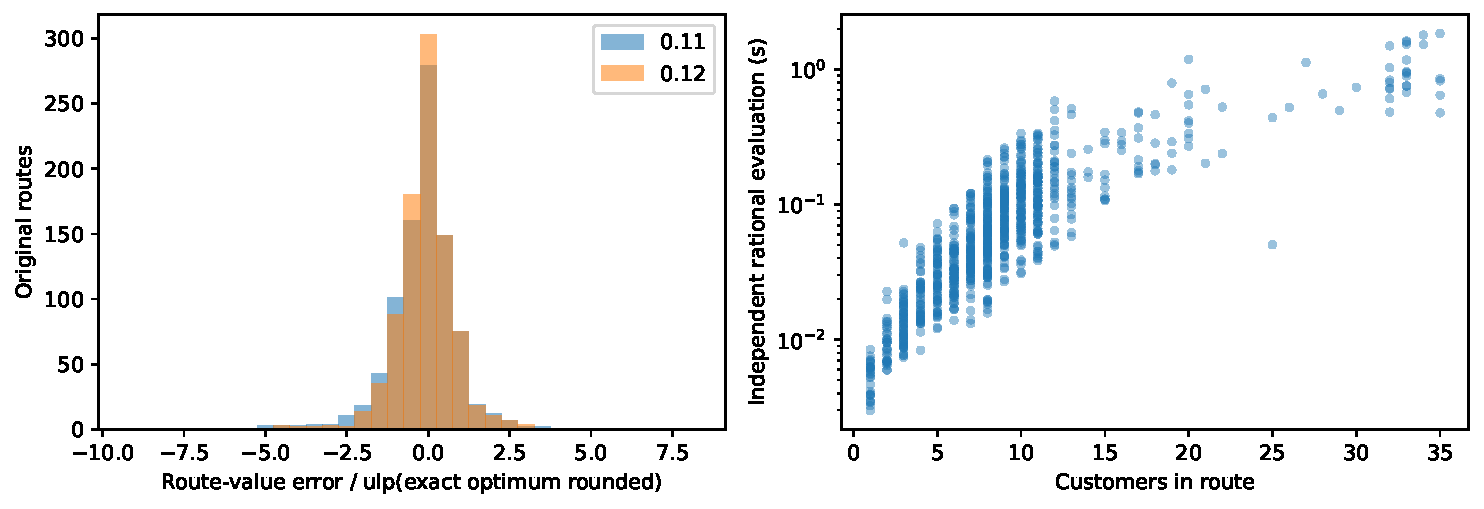
\includegraphics[width=\linewidth]{figures/original-error-runtime.pdf}
\caption{Original route-value error relative to the exact binary-operand optimum, in units of the binary64 spacing at its rounded value (left), and the independent rational evaluator's descriptive wall time against route length (right). Timings include the implementation described in Section~\ref{sec:protocol} and do not measure KAYROS performance.}\label{fig:original}
\end{figure}

The rational reference completes every original route under both input interpretations. The binary-operand and shortest-decimal models have different exact optimum values on 895 of the 898 routes, with different rounded values on 377. Their maximum absolute optimum difference is approximately $7.68\times10^{-12}$, and they agree on whole-route feasibility here. Thus choosing a rational implementation still requires choosing the input model. The largest recorded cut numerator/denominator length is 954 bits. These bit lengths concern the cut set, not every intermediate ordinate, and are a lower view of the implementation's exact arithmetic sizes. They demonstrate why rational arithmetic is more than a switch from double to a fixed-width integer, even on moderate route lengths.


\section{Stepwise examples and the broader TD store}\label{sec:td-store}

This section distinguishes a reproduced material step effect from the broader corpus measurements. For the published Rifki-30 regression route $[23,21,12,3,4,25,30,29]$, the old fold returns duration $1768$ at departure $1301$, and the newer fold returns $1743$ at departure $1341$. The independent rational optimizer returns $(1743,1341)$ on the frozen binary operands. This establishes improved fidelity on this fixed route and operational incompatibility between the contracts. It does not establish a new optimum over route sets.

A jump can amplify a small upstream time perturbation into a large cost change: if the arrival curve jumps by $J$ at $u$, the values at $u$ and just to its right can differ by nearly $J$. Without continuity or a local margin away from every event, a small interpolation-error bound gives no small downstream cost bound. A hard due date can turn the same branch change into rejection. The original computational recipe is still well-defined, but this is a substantive limitation when interpreted as a model of ideal feasible schedules.

\begin{table}[htbp]
\centering
\caption{Available canonical TD BKS records by normative family label. ``Changed'' compares old/new values on the same current routes and artifacts. ``Feasibility flips'' compares their nonempty-domain route-set verdicts.}\label{tab:td-store}
\begin{tabular}{lrrr}
\toprule
Family & Available records & Changed totals & Feasibility flips\\
\midrule
\tableinput tables/td-family.tex
\bottomrule
\end{tabular}
\end{table}

The full available corpus has \TDChanged{} old/new total differences and \TDFlips{} temporal feasibility flips on the current route sets. The largest absolute total difference is $25$. All available current records pass the structural checks and match their declared values under the newer recipe. Those counts differ in meaning from the campaign's cost-edit count, since the campaign also changed routes and left some declared values numerically unchanged. The 42 changed TD twin route sets improve their target-instance values under both frozen contracts. This comparison establishes a fixed-route improvement in the available target artifacts, not a proof of the full relaxation relationship or renewed optimality.

The broader exact panel completes all 243 routes in both interpretations, with no whole-route feasibility disagreement on that selection. Its largest cut bit length is 1,503 and largest cut count is 1,828. Table~\ref{tab:panel} reports the isolated variants. Binary-operand and shortest-decimal exact optimum values differ on 167 routes, with different rounded values on 118 and maximum absolute difference approximately $2.36\times10^{-11}$. Larger exact instances and solver pricing campaigns remain outside the completed panel.

\begin{table}[htbp]
\centering
\caption{Broader exact panel: 243 routes from 35 recorded strata. Rounded optimum agreement uses the binary-operand reference. Forward replay uses generic arc interpolation. Median fold times are descriptive wall times with Python setup included, measured during separate experiment runs with varying load. They are not a controlled comparison of production throughput.}\label{tab:panel}
\small
\begin{tabular}{lrrrr}
\toprule
Recipe & \shortstack{Rounded optimum\\matches} & \shortstack{Forward\\rejections} & \shortstack{Maximum\\absolute error} & \shortstack{Median fold\\seconds}\\
\midrule
\tableinput tables/panel-variants.tex
\bottomrule
\end{tabular}
\end{table}

The independent binary-rational evaluator's median wall time is approximately $0.058$ seconds per original route and $0.709$ seconds per broader-panel route. The longest broader-panel binary evaluation takes approximately $53.64$ seconds. The recorded float fold medians are below $0.001$ seconds on the original panel and below $0.004$ seconds on the broader panel, including setup. These observations support the oracle's use for verification at the measured sizes. They do not provide a controlled solver speed ratio or establish the cost of an optimized exact implementation.

The 168 targeted synthetic cases produce 1 whole-route feasibility disagreement and 11 additional exact-value disagreements for the original recipe, compared with 0 and 1 for the newer recipe. These count exact equality to the rational result, unlike the rounded-agreement tables. The class deliberately concentrates on known numerical mechanisms, so its disagreement frequencies should not be treated as empirical rates for a benchmark population.

The strict slope prototype is evaluated against the already computed independent references. Its purpose is to isolate the rounded guard's semantics. On the original panel it has 485 correctly rounded optimum matches and 21 generic-forward rejections, versus 494 and 25 for the published newer recipe. On the broader panel those optimum-match counts are 174 and 175. Thus a stricter primitive predicate can improve one criterion without improving every aggregate measure. It improves the primitive counterexample, while its effects on the measured solution panels are reported alongside the other variants. We do not extrapolate the targeted improvement to every canonical route or declare the prototype a superior normative checker from those counts alone.


\section{The static checker and incumbent ranking}\label{sec:static}

This section gives static routing equal attention because its arithmetic and policy changes are distinct from the TD fold. The ordinary checker loop is unchanged between releases: it traverses the submitted routes, adds every depot/customer arc into one accumulator and evaluates static time windows by earliest forward traversal. It starts time at $0$, adds travel, waits to ready time, compares exactly to due time, then adds service. At the return depot it adds travel and checks the depot window. We reproduce those operations rather than silently imposing a new departure policy.

\begin{algorithm}[htbp]
\caption{Static pricing and time-window validation in both releases}\label{alg:static}
\begin{algorithmic}[1]
\State $C\gets0$, served set $\gets\varnothing$
\For{route $r$ in submitted order}
  \State $i\gets0$, load $\gets0$, $t\gets0$
  \For{customer $j$ in $r$}
    \State Reject invalid/repeated customer or capacity overflow
    \State $C\gets C+c_{ij}$
    \If{time windows exist}
      \State $u\gets\max(t+c_{ij},e_j)$, reject if $u>l_j$, $t\gets u+s_j$
    \EndIf
    \State $i\gets j$
  \EndFor
  \State $C\gets C+c_{i0}$
  \State If windows exist, reject if $\max(t+c_{i0},e_0)>l_0$
\EndFor
\State Reject missing customers or exceeded fleet limit
\State Reject a declared cost unequal to $C$, otherwise return $C$
\end{algorithmic}
\end{algorithm}

For integer costs, Python integers remain exact. For floating costs, the loop is a flat sequential fold, without a per-route reset of the cost accumulator. The static helper \texttt{compute\_solution\_cost} instead computes each route subtotal and calls built-in \texttt{sum()} on those subtotals. Parenthesization can therefore differ from the checker even in one interpreter. Moreover, Python 3.12 changed the float \texttt{sum()} algorithm. Our positive witness $[10^{16},1,1]$ returns $10^{16}$ under 3.11's \texttt{sum()}, and $10^{16}+2$ under the tested 3.12--3.14 interpreters. The explicit left fold returns $10^{16}$ throughout. This is separate from the unchanged TD explicit total \autocite{pythonSum2026}.

The new static BKS store validates candidates, canonicalizes their route ordering for storage, and compares exact rational sums of \texttt{repr(float(arc\_cost))}. It still stores the ordinary checker value. Thus the ranking objective and the displayed/stored computational value are distinct. Exact decimal ranking removes permutation ties and, on symmetric matrices, reversal effects in the mathematical sum. It can be a sensible declared policy. It nevertheless changes the meaning of a strict incumbent improvement relative to binary64 checker scoring \autocite{mamutChecker0122026}.

\begin{table}[htbp]
\centering
\caption{Static sweep, available records only. Order sensitivity tests the submitted, canonical, reversed route-list and fixed-seed shuffled orders, with every route's internal direction unchanged. ``Grouped'' compares the helper's grouped accumulation with the flat checker in Python 3.13. ``Scale 1000'' requires every selected decimal-scaled arc and their total to be integral and within nonnegative signed 64-bit range.}\label{tab:static}
\begin{tabular}{lrrrr}
\toprule
Family & Available & Order-sensitive & Grouped differs & Scale 1000\\
\midrule
\tableinput tables/static-family.tex
\bottomrule
\end{tabular}
\end{table}

Every one of the \StaticComplete{} available static records passes the tagged structural/time-window checker and matches its declared cost. The tested permutations produce differing totals for \StaticOrdering{} records, and the grouped helper differs for \StaticHelper{}. Neither phenomenon alone proves that a prescribed flat-checker computation is wrong. It does show that routing the same solution through an alternative helper or reduction order can break exact comparisons. The independent binary-rational and decimal-rational temporal traversals do not flip feasibility for any of these available stored route sets. The constructed $0.1+0.2$ at deadline $0.3$ example does distinguish decimal-exact from binary64/binary-rational feasibility, so absence of flips in this corpus is not a general equivalence claim.

The 31 restored Mamut2026 records are exact decimal ties on their route arc sums. Under canonical flat binary64 scoring, 11 restored current route sets are worse than their campaign predecessors, 4 are better and 16 tie. The separate Poryos static twin replacement improves both metrics. These observations establish that the audit's tie label is policy-dependent. They do not establish that all 31 should be restored or removed under every possible policy. A hierarchical objective also compares route count before its secondary cost, and that tier must remain explicit.

\begin{figure}[htbp]
\centering
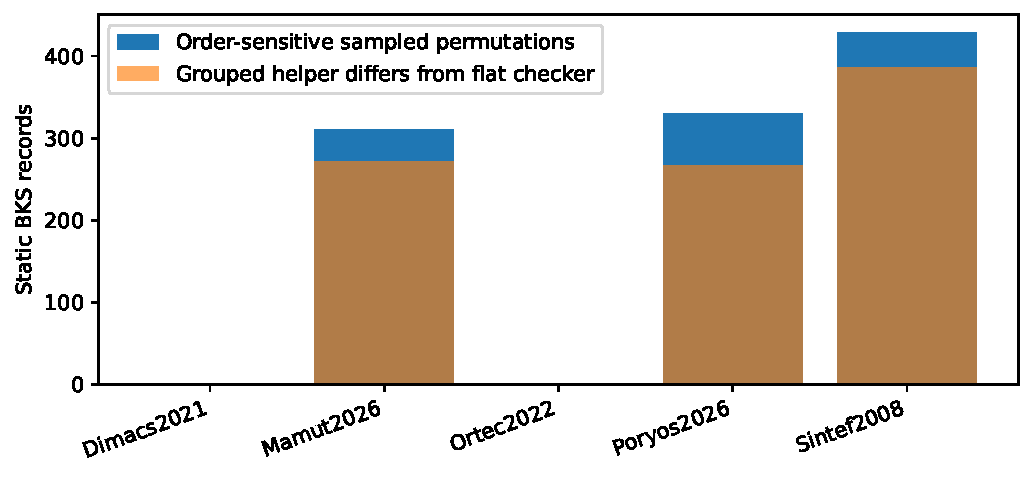
\includegraphics[width=0.85\linewidth]{figures/static-ordering.pdf}
\caption{Static ordering and grouped-helper effects in the available store. These are measurements of different computational reductions on fixed route sets, not changes to their exact arc multisets.}
\end{figure}

The scale-1000 eligibility test passes for \StaticScaled{} records. It fails for the full-precision Sintef2008 costs, whose decimal spellings generally require finer scales. This test checks every selected route arc and the complete arc-sum objective, not every matrix entry, solver penalty, service time or intermediate arithmetic. An integral total alone would be insufficient, since fractions of a scaled unit can cancel in a sum. The \texttt{fsum} experiment offers a more accurate reduction of binary operands, but is a different cost recipe and inherits platform caveats documented by Python. A correctly rounded sum of exact binary operands and an exact sum of decimal spellings are also different proposals \autocite{pythonFsum2026}.

The submitted flat total matches the correctly rounded exact binary-operand sum on 1,037 of 1,956 records. Canonical flat ordering gives 1,022 matches, grouped route reduction gives 1,672, and \texttt{fsum} gives 1,956 on this host and panel. Canonical ordering therefore provides deterministic storage order, without guaranteeing greater summation accuracy. The rounded exact binary and decimal sums differ on 39 records, further distinguishing a binary-operand reduction proposal from the newer decimal ranking policy.


\section{Consequences of the September change campaign}\label{sec:campaign}

This section separates numerical migration effects from independent integrity repairs. The pinned diff contains 928 BKS cost edits, of which 870 concern TD records and 58 static records, and 74 route-list edits. Of the latter, 43 are twin replacements (42 TD and 1 static) and 31 are the Mamut restorations discussed above. The original audit ledger's numerical claims need to be interpreted under their chosen ranking/feasibility metric, rather than treated as contract-neutral descriptions.

We independently confirm 210 changed optimality metadata records. Their changed keys are \texttt{note} and \texttt{proven\_optimum}. The notes acknowledge repricing from \contractone{} to \contracttwo{}, leave the prover's dual bound as a historical value and state that recertification is pending. The \texttt{proven} flag is retained. This creates mixed metadata if read without its note: a repriced incumbent value appears next to an older-contract proof claim. We should preserve the original evidence and attach the proof to its original contract, rather than erase it or infer a new proof from the repriced route set.

Twin relationships require their own care. Capacity-equivalent removal of a hard constraint preserves the usual exact-model containment, but a specialized computational recipe may evaluate two structurally related instance types through different operations. In particular, replacing waiting windows by an unrestricted service chain can itself change roundoff. We should test the claimed operational relaxation relationship under the chosen checker, even when the mathematical relaxation is sound. The newer objective-aware screen and depot-window check address real modeling issues, but cross-evaluated incumbents must be evaluated under each target's declared contract before any replacement policy is chosen.

\begin{table}[htbp]
\centering
\caption{Disposition classes for the 24 audit campaign resolutions. These are recommendations for separating a later repair/migration decision, not changes performed by this investigation. A sanitized source-path and disposition map accompanies the public evidence. The original audit ledger remains private.}\label{tab:disposition}
\begin{tabularx}{\linewidth}{>{\raggedright\arraybackslash}p{0.23\linewidth}>{\raggedright\arraybackslash}X}
\toprule
Change group & Investigation conclusion\\
\midrule
TD fold and repricing & Treat as a contract migration. Preserve both recipes, original declared values and original certificates. A fidelity gain on stepwise examples does not establish nonconformance to the old recipe.\\
Static decimal ranking and 31 restorations & Treat exact decimal ranking as a separate policy choice. Retain candidate validation and canonical storage as independently reviewable changes. Reassess incumbent choices using the adopted objective.\\
Twin replacements and objective-aware checks & Preserve candidates and cross-evaluation evidence. Validate target-specific timing, depot windows, objective and route constraints under each contract before selecting incumbents.\\
Sidecar hashes, atomic/staged writes and regeneration & These address provenance, stale data and partial publication independently of the choice of route arithmetic. We recommend retaining the repairs subject to their own regression evidence.\\
Instance identifiers, archive layout, exception handling and cost reporting & These address discovery and interface consistency. A blanket rollback would remove useful repairs. Keep them separable from numerical migration.\\
Export guards, site sorting, payload handling and download selection & These address mismatched exported instances and interface/integrity defects. Their retention does not require adopting \contracttwo{}.\\
\bottomrule
\end{tabularx}
\end{table}

The source review establishes separability and the documented reasons for these repairs. It is not a fresh security audit or an exhaustive verification of the tools' generation semantics. In particular, changing feasible anchors or generated time windows changes instance generation and should retain its generator/version provenance, even if the algorithm fixes a practical failure. We do not roll those changes into a numerical-checker conclusion.

We identify a concrete cascading compatibility issue in the tools' legacy run handling: schema-1 runs are revalidated under the installed checker, but a changed verdict or cost is described as instance regeneration. Its cached legacy validation is keyed by instance hash without a checker-contract identifier. The newer schema records instance bytes but does not itself identify the evaluation contract. Hence unchanged instance bytes can coexist with a changed computational interpretation, and reverting or upgrading a checker can leave cached legacy status inappropriate. This should be handled as an explicit contract compatibility condition, preserving the original run and evaluator identity.

The reviewed staging repair is atomic per file with a recovery marker and roll-forward behavior, not one simultaneous atomic swap of an entire collection. The archive repair also still replaces an existing release-stamped subtree when fetching again, so its mitigation does not by itself preserve locally added BKS inside that subtree. These limits should remain visible when retaining the independent integrity repairs.


\section{Literature and historical choices}

This section locates the investigated recipes within the literature without attributing a finite arithmetic specification to papers that describe an exact mathematical operation. \textcite{visserEfficientMoveEvaluations2020} use ready-time functions and composition for route evaluation and efficient neighborhood search. Their tree constructions exploit mathematical associativity. This does not establish bitwise associativity of a binary64 implementation. An authoritative sequential fold can therefore coexist with faster solver structures, provided accepted results return to the prescribed fold.

\textcite{blauthVehicleRoutingTimedependent2024} formulate continuous, nondecreasing piecewise-linear arrival-time functions and efficient operations, including scheduling. Their mathematical results provide a useful model and complexity context. They do not select the particular binary64 waiting-map interpolation or specialized arithmetic of either investigated release. Genuine jumps require an additional point/side convention. We preserve the canonical data's smallest ordinate at an exact repeated abscissa rather than assuming that a vertical chain connector is a continuum of possible arrival values.

\textcite{lera-romeroLinearEdgeCosts2020} investigate labeling algorithms with linear edge costs and discuss the importance of implementation choices to numerical experiments. \textcite{dabiaErratumBranchPrice2024} correct implementation results associated with the earlier branch-and-price work. These sources motivate careful validation, but do not establish that our original checker must be replaced by one particular arithmetic refinement. The 146 original solution records provide a concrete historical panel for our own comparison \autocite{dabiaBranchPriceTimeDependent2013}.

An adjacent literature demonstrates that exact rational piecewise-affine software is a realistic option. \textcite{zippoPseudoInverseComposition2023} explicitly separate point elements and open segments when handling discontinuities. \textcite{zippoNancy2022} implement rational arithmetic with arbitrary-size integers to avoid overflow, with a finite-width alternative for performance. This supports investigating exact references and bit complexity. It does not imply that a rational implementation fits the throughput or integration requirements of KAYROS without a dedicated comparison.

Static routing has a related trade-off. Scaling and rounding alter the finite instance, as our earlier VRPTW study investigates. PyVRP's issue \#623 discusses fractional cost modeling and integer range concerns, and its September 27, 2026 PR \#1196 proposes returning to floats. The initial investigation captured the PR before its merge. It was merged on September 30, 2026, and we update its status here. We use this as evidence that the trade-off remains practical, without interpreting a project discussion as a universal performance result or a recommendation to copy its design \autocite{rascoussierImpactScalingRounding2026,woudaDoubles2024,woudaFloats2026}.


\section{Original solution totals}\label{app:originals}

This appendix records the original declared total and both contract totals for every original solution. Decimal strings are round-trip representations. The last column counts binary64 representable-value steps between the old and new totals, so small changes remain visible even when neighboring printed values look similar. These are fixed-route evaluations, not renewed optimality claims.

\begingroup
\scriptsize
\setlength{\tabcolsep}{3pt}
\setlength{\parskip}{0pt}
\setlength{\LTpre}{0pt}
\setlength{\LTpost}{0pt}
\begin{longtable}{lrrrrr}
\caption{All 146 original Lera-Romero solution totals.}\\
\toprule
Instance & Routes & Published & 0.11 & 0.12 & ULP steps\\
\midrule
\endfirsthead
\toprule
Instance & Routes & Published & 0.11 & 0.12 & ULP steps\\
\midrule
\endhead
\bottomrule
\endfoot
\tableinput tables/original-solutions.tex
\end{longtable}
\endgroup


\section{Finite-input models and portability}\label{app:models}

This appendix provides the detailed input-model and reproducibility distinctions behind the main comparison.

\subsection{The finite input model}

A finite binary64 value is an exact dyadic rational, so an independent rational model can preserve the stored floating-point operands exactly. A decimal interpretation instead treats the shortest decimal representation as exact. For example, \texttt{Fraction(0.1)} and \texttt{Fraction("0.1")} denote different rationals. Neither reconstructs an unrounded Euclidean distance, and neither establishes the physical truth of a road travel-time estimate. Our TD references operate on materialized, frozen arrival-time breakpoints. The decimal TD reference uses their shortest round-trip decimal spellings, not an assertion that the original raw sidecar tokens or an ideal materializer denoted those exact decimals \autocite{pythonFraction2026}.

We consequently separate 2 exact questions: the ideal piecewise-affine route defined by the binary operands, and the ideal piecewise-affine route defined by these decimal interpretations. Replacing the finite input model is different from changing the arithmetic on the same operands. This distinction also matters in static routing, where rounding a distance before summation and rounding its final sum define different objectives.

\subsection{Conformance, fidelity and reproducibility}

\emph{Operational conformance} means reproducing the prescribed finite computation. \emph{Mathematical fidelity} means proximity to a separately specified exact model, including its branch and feasibility decisions. \emph{Reproducibility} means obtaining the same contract result from the same artifacts and recipe. A deterministic algorithm can have low fidelity at a discontinuity, and a more accurate algorithm can break historical conformance. These properties should be measured separately.

Binary64 alone does not specify a recipe: parenthesization, intermediate rounding and fused operations matter. Our C++ diagnostic uses $a=1+2^{-27}$, $b=1-2^{-27}$ and $c=-1$. A separately rounded product followed by addition returns $0$, while a fused multiply-add returns $-2^{-54}$. Both use floating-point hardware. A portable checker standard therefore fixes the operation sequence, rounding mode and contraction/reassociation policy, together with treatment of nonfinite and exceptional inputs. The reproduced examples use finite normal-range data \autocite{goldbergFloatingPoint1991}.

\subsection{The role of a reference checker}

A simple binary64 reference has practical value: solvers can port its operations, accepted moves can be repriced cheaply, and readers can audit one fixed recipe. Our prior KAYROS work deliberately places the checker above optimized move-evaluation structures and compares declared costs exactly. The manuscript and KAYROS reports describe sequential unnormalized composition and canonical TD summation as the standard. Their claims concern this prescribed computation and named solver assumptions. They do not imply unrestricted exact real arithmetic \autocite{rascoussierKAYROSAnytimeExact2026,rascoussierKAYROSTechReport2026}.

Changing that authority affects more than final cost strings: move acceptance, incumbent ranking, feasibility, lower bounds, reference gaps and anytime scores may all change. Prior comparisons with explicit reference policies remain evidence about the contract and reference snapshot that they used. A new checker value cannot be substituted into a historical result without revisiting that context \autocite{rascoussierAnytimeSolverEvaluation2026,rascoussierHexalyThreadScaling2026}.


\section{Provenance and reproduction}\label{app:reproduction}

This appendix records the frozen sources and distribution checks, together with the evidence needed to reproduce the numerical comparisons. The public repository provides the executable code, compact TD input panels, historical static arc operands and archived route-level results. It retains upstream source and data licenses, while excluding personal discussions and the original private audit ledger \autocite{onyrInvestigation2026}.

The source commits are \texttt{425dff3} for 0.11.0 and \texttt{a9f7d9a} for 0.12.0. Annotated tag objects are recorded separately from their peeled source commits. The original corpus comparison uses MAMUT-routing baseline \texttt{93d9cc4} and snapshot \texttt{0d48b4f}, with 11 satellite baseline/snapshot pairs. These pins remain the authority for the original numerical results. Later static comparisons require identical instance bytes and report their candidate source revisions separately.

We download the published PyPI wheels into an isolated evidence cache, verify their advertised SHA-256 digests and compare their package Python files without installing them. All 23 files for 0.11.0 and all 25 for 0.12.0 match the corresponding frozen source exactly. Distribution URLs, hashes and upload timestamps appear in \path{manifests/distributions.json}. Hence the studied sources represent the published recipes, rather than an assumed tag-to-wheel correspondence.

The library and tools default branches contain no source changes beyond the frozen audited releases at the October 14 inspection. The newer main MAMUT-routing revision \texttt{6419553} changes its Mamut2026 submodule pin for a reported third BKS campaign. The pinned satellite revision \texttt{c62eca8} was unavailable from the satellite remote, whose advertised HEAD was \texttt{4715692}. We therefore exclude that campaign from numerical conclusions. Its absence does not alter results on the frozen corpus, but prevents describing that corpus as the latest published store. \path{manifests/recent-changes.json} records the inspection.

Historical source inspection dates the generic TD module to July 2, 2026. The fixed-cost duration objective was added in July and horizon/ready-time construction changed in August. Our reference to the historical protocol concerns generic sequential composition, specifically the frozen 0.11 implementation, not byte-identical behavior of every earlier release.

The original investigation used a private 180-entry audit ledger as contextual evidence and reviewed 24 resolved items against pinned sources. We do not claim a new independent verification of all audit assertions. The public disposition map preserves the source paths, conclusions and review limits without publishing that ledger. Independent numerical measurements are distinguished from contextual audit claims.

The principal numerical evidence comprises \path{results/original-solutions.csv}, \path{results/original-routes.csv}, \path{results/static-solutions.csv}, \path{results/td-solutions.csv}, \path{results/td-replacements.csv}, \path{results/summary.json}, \path{results/static-history.json}, and the controlled timing JSON files. The archives in \path{data} restore the exact-panel inputs and all original route-result records. The bundle verifier checks their manifests and the frozen source hashes. Full-store materialized inputs require the pinned external repositories and their sidecars. Missing-input and source-sidecar manifests retain the coverage gaps.

From a clean checkout, run \texttt{uv sync --locked}, \texttt{uv run python -m ncci.bundle restore}, and \texttt{uv run pytest -q}. The repository README gives commands for candidate comparisons, conformance, controlled timings, table regeneration and the pdflatex/biber build. Timing reruns are host-specific. The report does not require private discussions or the audit ledger to reproduce its numerical comparisons.
